\section{Appendix: Near Detector and Uncertainties}\label{sec:nu-osc-12}\label{sec:physics-lbnosc-ND-app}

The DUNE near detector (ND) will be located 574 m from the neutrino target at Fermilab and approximately 60 m underground. The hall is oriented at 90 degrees with respect to the beam axis to facilitate measurements at both on-axis and off-axis locations. The detector concept consists of a liquid argon time-projection chamber (LAr TPC) functionally coupled to a magnetized multi-purpose tracker (MPT). The MPT includes a high-pressure gaseous argon (HPG) TPC, surrounded by an electromangetic calorimeter (ECal), and a magnet. More details on the design can be found in Chapter~\ref{ch:ndexecutivesummary}.

The LAr TPC is a modular detector with pixelated readout, based on the concept being studied by the Argon Cube collaboration~\cite{ArgonCube}, and is the most upstream component of the ND. Each module is itself a LAr TPC with two anode planes and a central cathode. The active dimensions are $1 \times 3 \times 1$~m ($x \times y \times z$), where the $z$ direction is $6^{\circ}$ upward from the neutrino beam, and the $y$ direction points upward. Charge drifts in the $\pm x$ direction, with a maximum drift distance of 50 cm for electrons created in the center of a module. The module design is described in detail in Ref.~\cite{ArgonCube}. The full LAr detector consists of an array of modules in a single cryostat. The minimum active size for full containment of hadronic showers is $3 \times 4 \times 5$~m. High-angle muons can also be contained by extending the width to 7 m. For this analysis, 35 modules are arranged in an array 5 modules deep in the $z$ direction and 7 modules across in $x$ so that the total active dimensions are $7 \times 3 \times 5$~m. The total active LAr volume is $105 m^{3}$, corresponding to a mass of 147 tons.

The anode planes are tiled with readout pads, such that the $yz$ coordinate is given by the pad location and the $x$ coordinate is given by the drift time, and the three-dimensional position of an energy deposit is uniquely determined. A dedicated, low-power readout ASIC is being developed, which will enable single-pad readout without analog multiplexing~\cite{LArPix}. The module walls orthogonal to the anode and cathode are lined with a photon detector that is sensitive to scintillation light produced inside the module, called ArCLight~\cite{ArCLight}. The detector is optically segmented, and tiled so that the vertical position of the optical flash can be determined with $\sim$30 cm resolution. It is therefore possible to isolate flashes to a volume of roughly 0.3 m$^{3}$, and associate them to a specific neutrino interaction even in the presence of pile-up. The neutrino interaction time, $t_{0}$, is determined from the prompt component of the scintillation light.

% exact dimensions of PV in simulation are 273cm radius, 518cm axis
The MPT sits immediately downstream of the LAr TPC so that in the on-axis position, the beam center crosses the exact center of both the LAr and HPG active volumes. The HPG TPC is cylindrical, approximately 5 m in diameter and 5 m long, and will reuse existing readout chambers from the ALICE experiment. It is divided into two drift regions by a central cathode, and filled with a 90/10 Ar/CO$_{2}$ gas mixture, pressurized to 10 atmospheres. The gas TPC is described in detail in Ref.~\cite{gasTPC}. It is surrounded by a cylindrical pressure vessel and a highly granular, tiled ECal. The ECal is composed of a series of absorber layers, followed by arrays of scintillator tiles. Each tile is read out by a SiPM mounted to a 1 mm thick printed circuit board. The ECal design is described in Ref.~\cite{CALICEecal}. The entire MPT is inside a magnetic field with a central field strength of 0.4 T. The reference magnet design is a conventional dipole, described in the DUNE CDR~\cite{Acciarri:2016ooe}. Solenoid and superconducting coil designs are also being considered.

For the oscillation sensitivity analysis presented in this document, the pressure vessel is assumed to be 3 cm titanium. The ECal tiles are $10 \times 10 \times 5$~mm, with a 2 mm copper absorber. The inner-most 10 ECal layers are inside the pressure vessel, giving excellent angular resolution to photon-induced showers, which generally do not convert in the gas. An additional 20 ECal layers are positioned outside the pressure vessel to contain energy from these showers. The magnet is a solenoid with an inner radius of 320 cm and total length along the cylinder axis of 780 cm. The yoke is cut out in the upstream barrel to minimize the passive material between the two TPC detectors. A profile view visualization of the ND is shown in Figure~\ref{fig:NDvis}.

\begin{dunefigure}[ND visualization]{fig:NDvis}
{The near detector shown from the side. The neutrinos are incident from the left along the axis shown, which intersects the center of the LAr and GAr detectors.}
 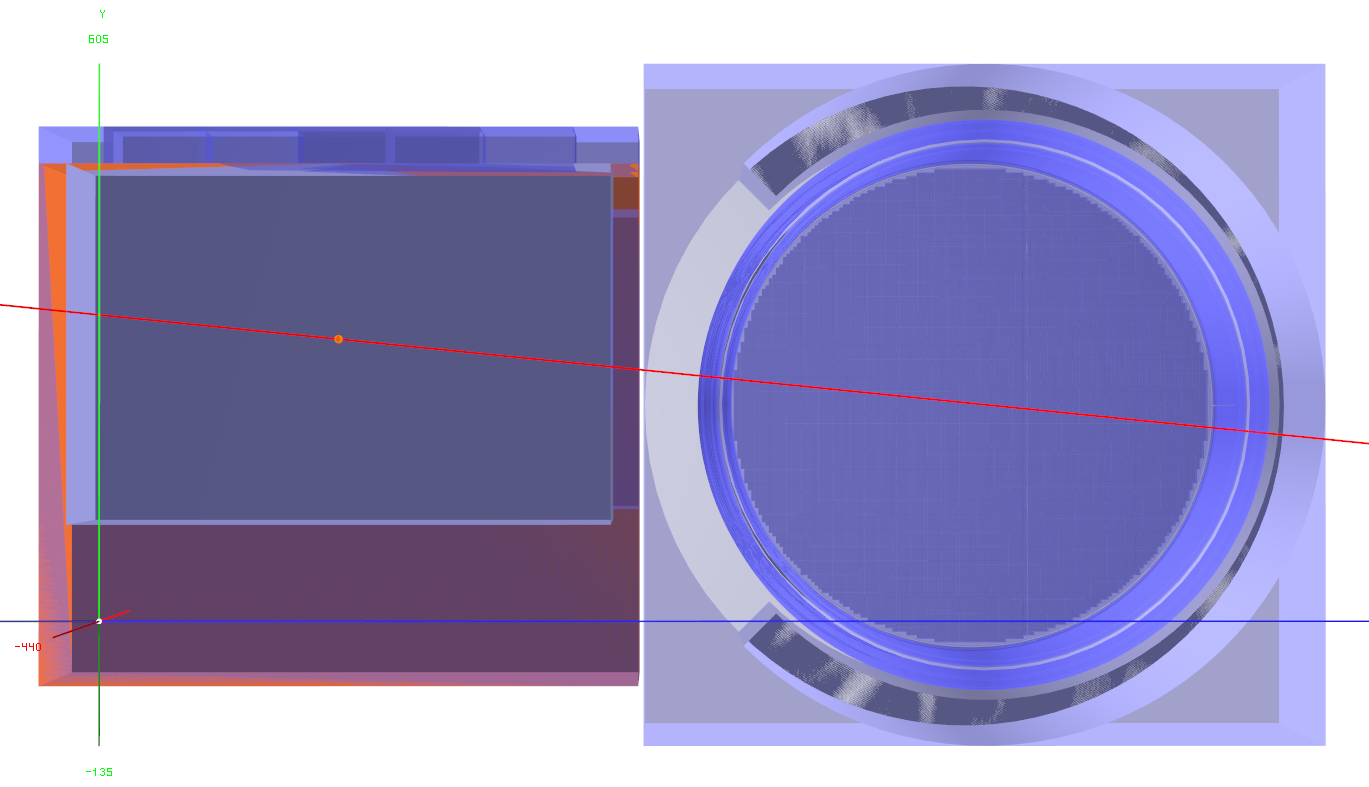
\includegraphics[width=0.6\textwidth]{lar_mpt_in_hall.png}
\end{dunefigure}

Liquid argon events are required to originate in a fiducial volume that excludes 50 cm from the sides and upstream edge, and 150cm from the downstream edge of the active region, for a total of $6 \times 2 \times 3$~m$^{2}$. A hadronic veto region is defined as the outer 30 cm of the active volume on all sides. Events with more than 30 MeV total energy deposit in the veto region are excluded from analysis, as this energy near the detector edge suggests leakage, resulting in poor energy reconstruction. Even with the containment requirement, events with large shower fluctuations to neutral particles can still be very poorly reconstructed. Neutrons, in particular, are largely unreconstructed energy.

Electrons are reconstructed calorimetrically in the liquid argon. The radiation length is 14 cm in LAr, so for fiducial interactions there are between 10 and 30 radiation lengths between the vertex and the edge of the TPC. As there is no magnetic field in the LAr TPC region, electrons and positrons cannot be distinguished and the selected $\nu_{e}$ sample contains both neutrino- and antineutrino-induced events.

Muons with kinetic energy greater than $\sim$1 GeV typically exit the LAr. An energetic forward-going muon will pass through the ECal and into the gaseous TPC, where its momentum and charge are reconstructed by curvature. For these events, it is possible to differentiate between $\mu^{+}$ and $\mu^{-}$ event by event. Muons that stop in the LAr or ECal are reconstructed by range. Exiting muons that do not match to the HPG TPC are not reconstructed, and events with these tracks are rejected from analysis. The asymmetric transverse dimensions of the LAr volume make it possible to reconstruct wide-angle muons with some efficiency. High-angle tracks are typically lost when the $\nu-\mu$ plane is nearly parallel to the $y$ axis, but are often contained when it is nearly parallel to the $x$ axis. 

The charge of stopping muons in the LAr volume cannot be determined. However, the wrong-sign flux is predominantly concentrated in the high-energy tail, where leptons are likelier to be forward and energetic. In FHC mode, the wrong-sign background in the focusing peak is negligibly small, and $\mu^{-}$ is assumed for all stopping muon tracks. In RHC mode, the wrong-sign background is larger in the peak region. Furthermore, high-angle leptons are generally at higher inelasticity, which enhances the wrong-sign contamination in the contained muon sample. To mitigate this, a Michel electron is required. The wrong-sign $\mu^{-}$ captures on Ar with 75\% probability, effectively suppressing the relative $\mu^{-}$ component by a factor of four.

Events are classified as either $\nu_{\mu}$ CC, $\bar{\nu}_{\mu}$ CC, $\nu_{e}$+$\bar{\nu}_{e}$ CC, or NC. True muons and charged pions are evaluated as potential muon candidates. The track length is determined by following the true particle trajectory until it hard scatters or ranges out. The particle is classified as a muon if its track length is at least 1 m, and the mean energy deposit per centimeter of track length is less than 3 MeV. The mean energy cut rejects tracks with detectable hadronic interactions. The minimum length requirement imposes an effective threshold on true muons of about 200 MeV kinetic energy, but greatly suppresses potential NC backgrounds with short, non-interacting charged pions.

True electrons are reconstructed with an ad-hoc efficiency that is zero below 300 MeV, and rises linearly to unity between 300 and 700 MeV. Neutral-current backgrounds arise from photon and $\pi^{0}$ production. Photons are misreconstructed as electrons when the energy deposit per centimeter in the first few cm after conversion is less than 4 MeV. This is typically for Compton scatters, and can also occur due to a random downward fluctuation in the $e^{+}e^{-}$ dE/dx. The conversion distance must also be small so that no visible gap can be identified. We consider a photon gap to be clear when the conversion distance is greater than 2cm, which corresponds to at least three pad widths. For $\pi^{0}$ events, the second photon must also be either less than 50 MeV, or have an opening angle to the first photon less than 10 mrad. It is possible for CC $\nu_{\mu}$ events to be reconstructed as CC $\nu_{e}$ when the muon is too soft and a $\pi^{0}$ fakes the electron.

LAr events are classified as $\nu_{\mu}$ CC, $\bar{\nu}_{\mu}$ CC, $\nu_{e}$ + $\bar{\nu}_{e}$ CC, or NC. Charged-current events are required to have exactly one reconstructed lepton of the apropriate flavor. The muon-flavor samples are separated by reconstructed charge, but the electron sample is combined because the charge cannot be determined. The neutral-current sample includes all events with zero reconstructed leptons.

Events with exiting tracks that do not enter the HPG TPC are rejected. These are predominantly muon CC, where the muon momentum cannot be determined. Events with more than 30 MeV of visible hadronic energy in the veto region are also excluded. Reconstructed neutrino energy spectra for selected events are shown in Figure~\ref{fig:recoEvcats}.

\begin{dunefigure}[ND selected samples]{fig:recoEvcats}
{Reconstructed neutrino energy for events classified as $\nu_{\mu}$ CC, $\nu_{e}$ CC, and NC in FHC mode. The colors correspond to true neutrino flavor.}
 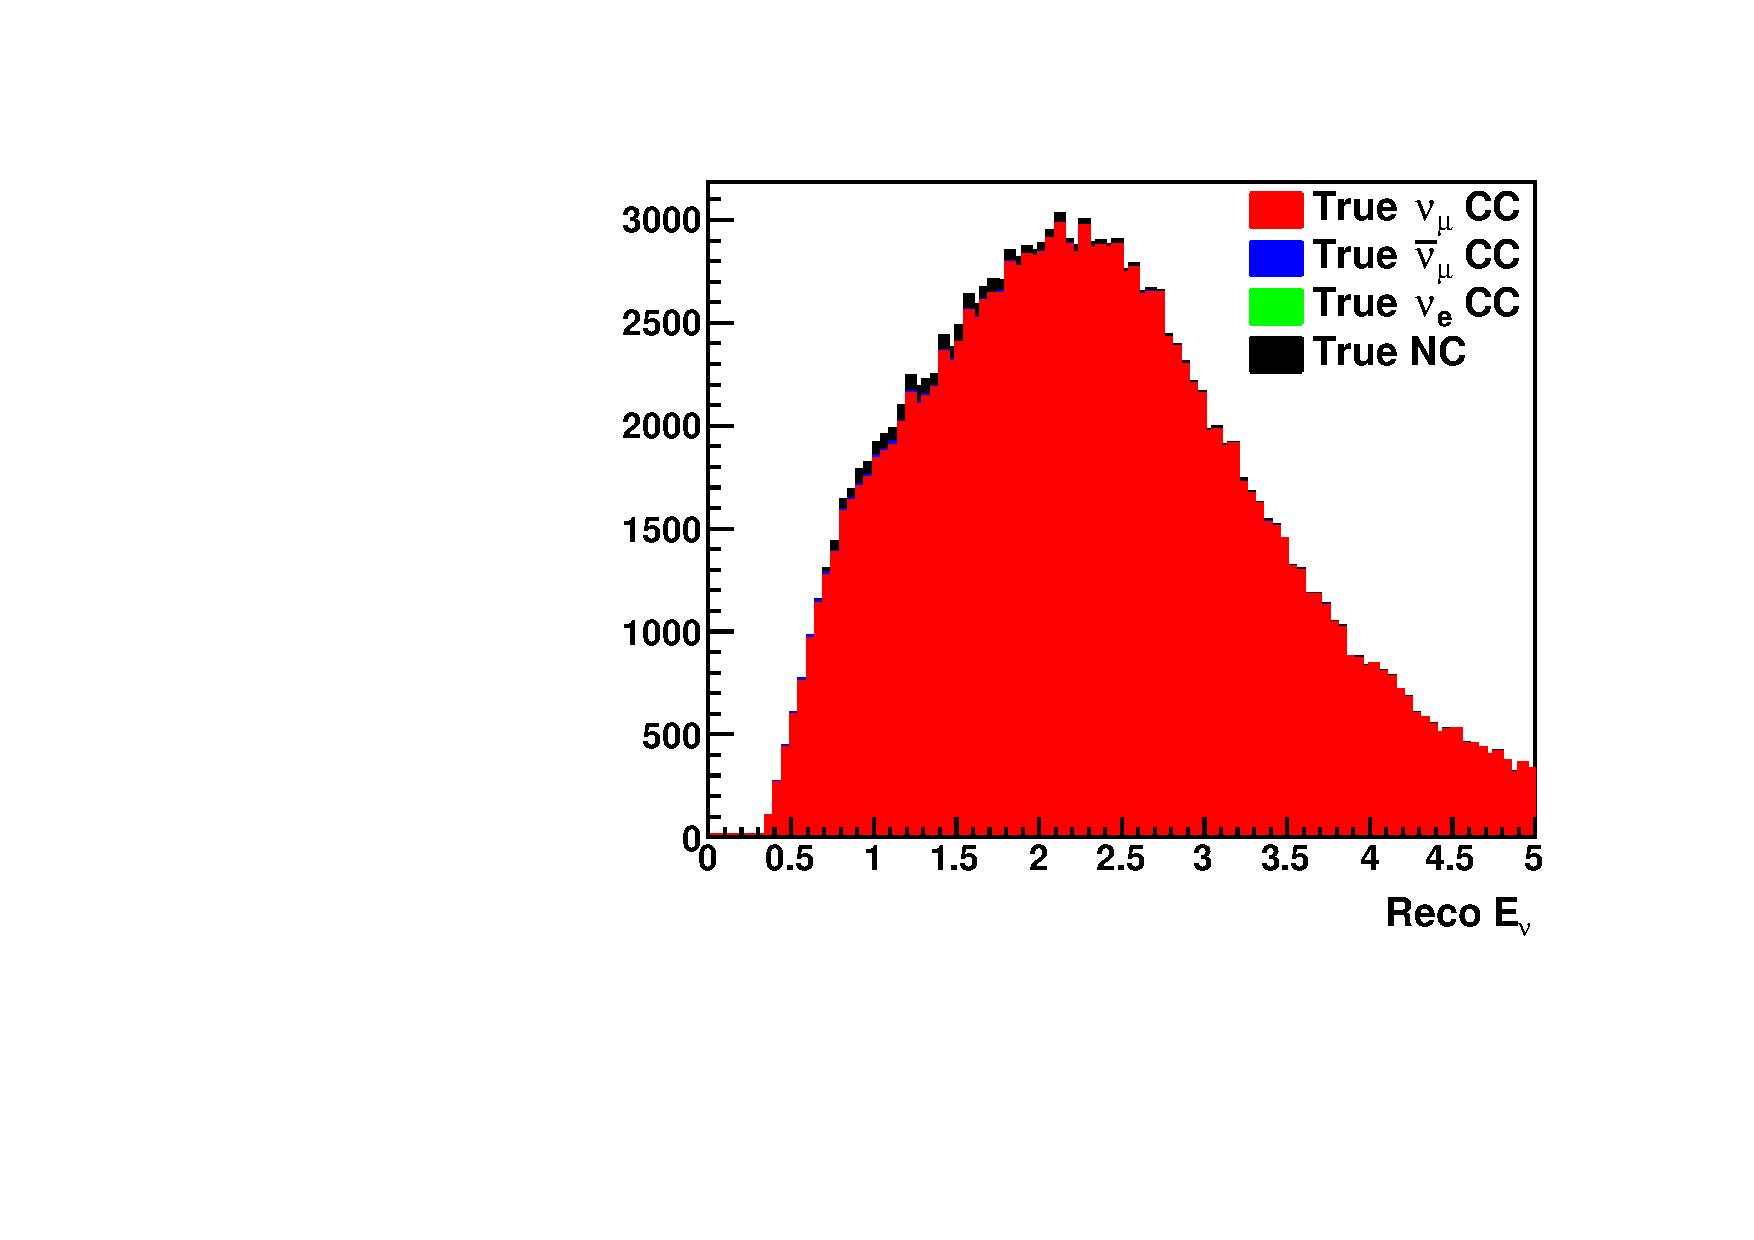
\includegraphics[width=0.3\textwidth]{recoE_muCC.pdf}
 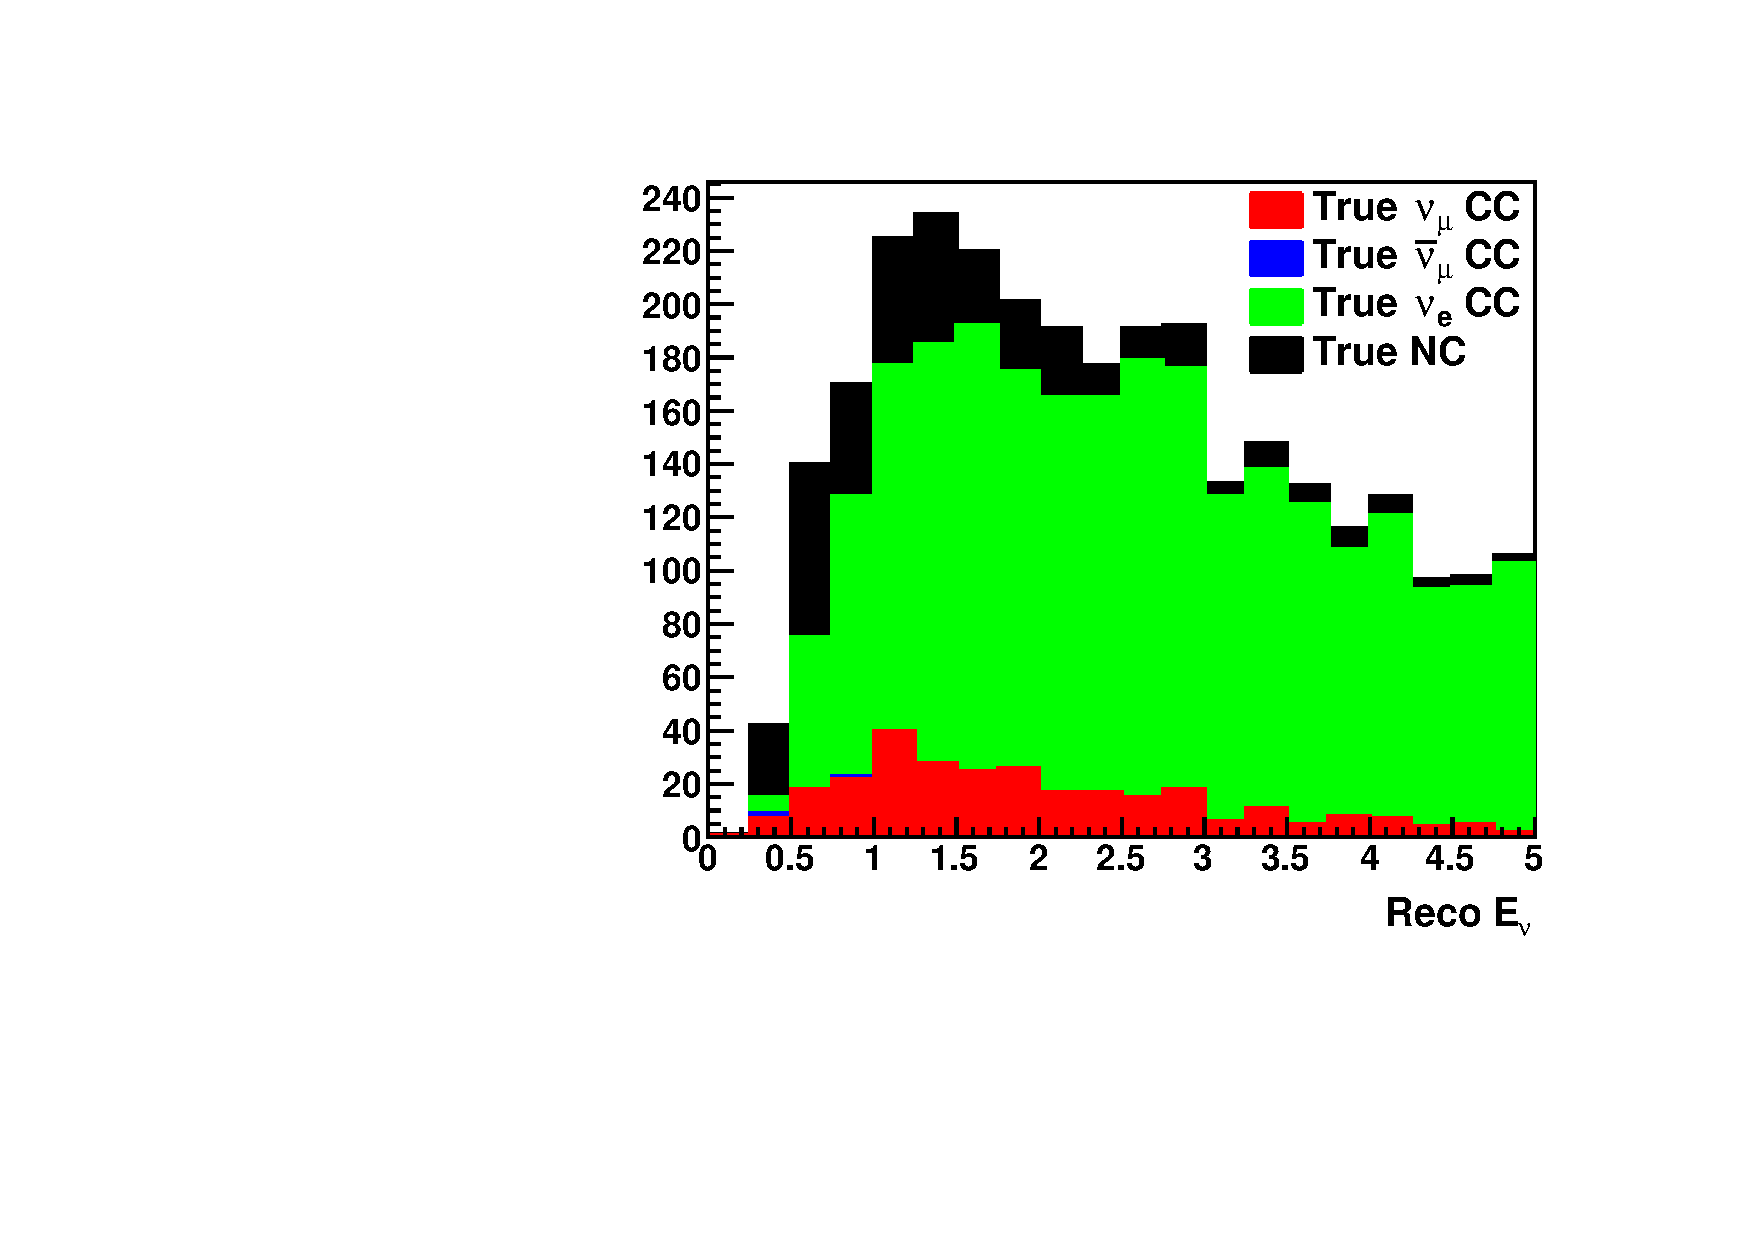
\includegraphics[width=0.3\textwidth]{recoE_eCC.pdf}
 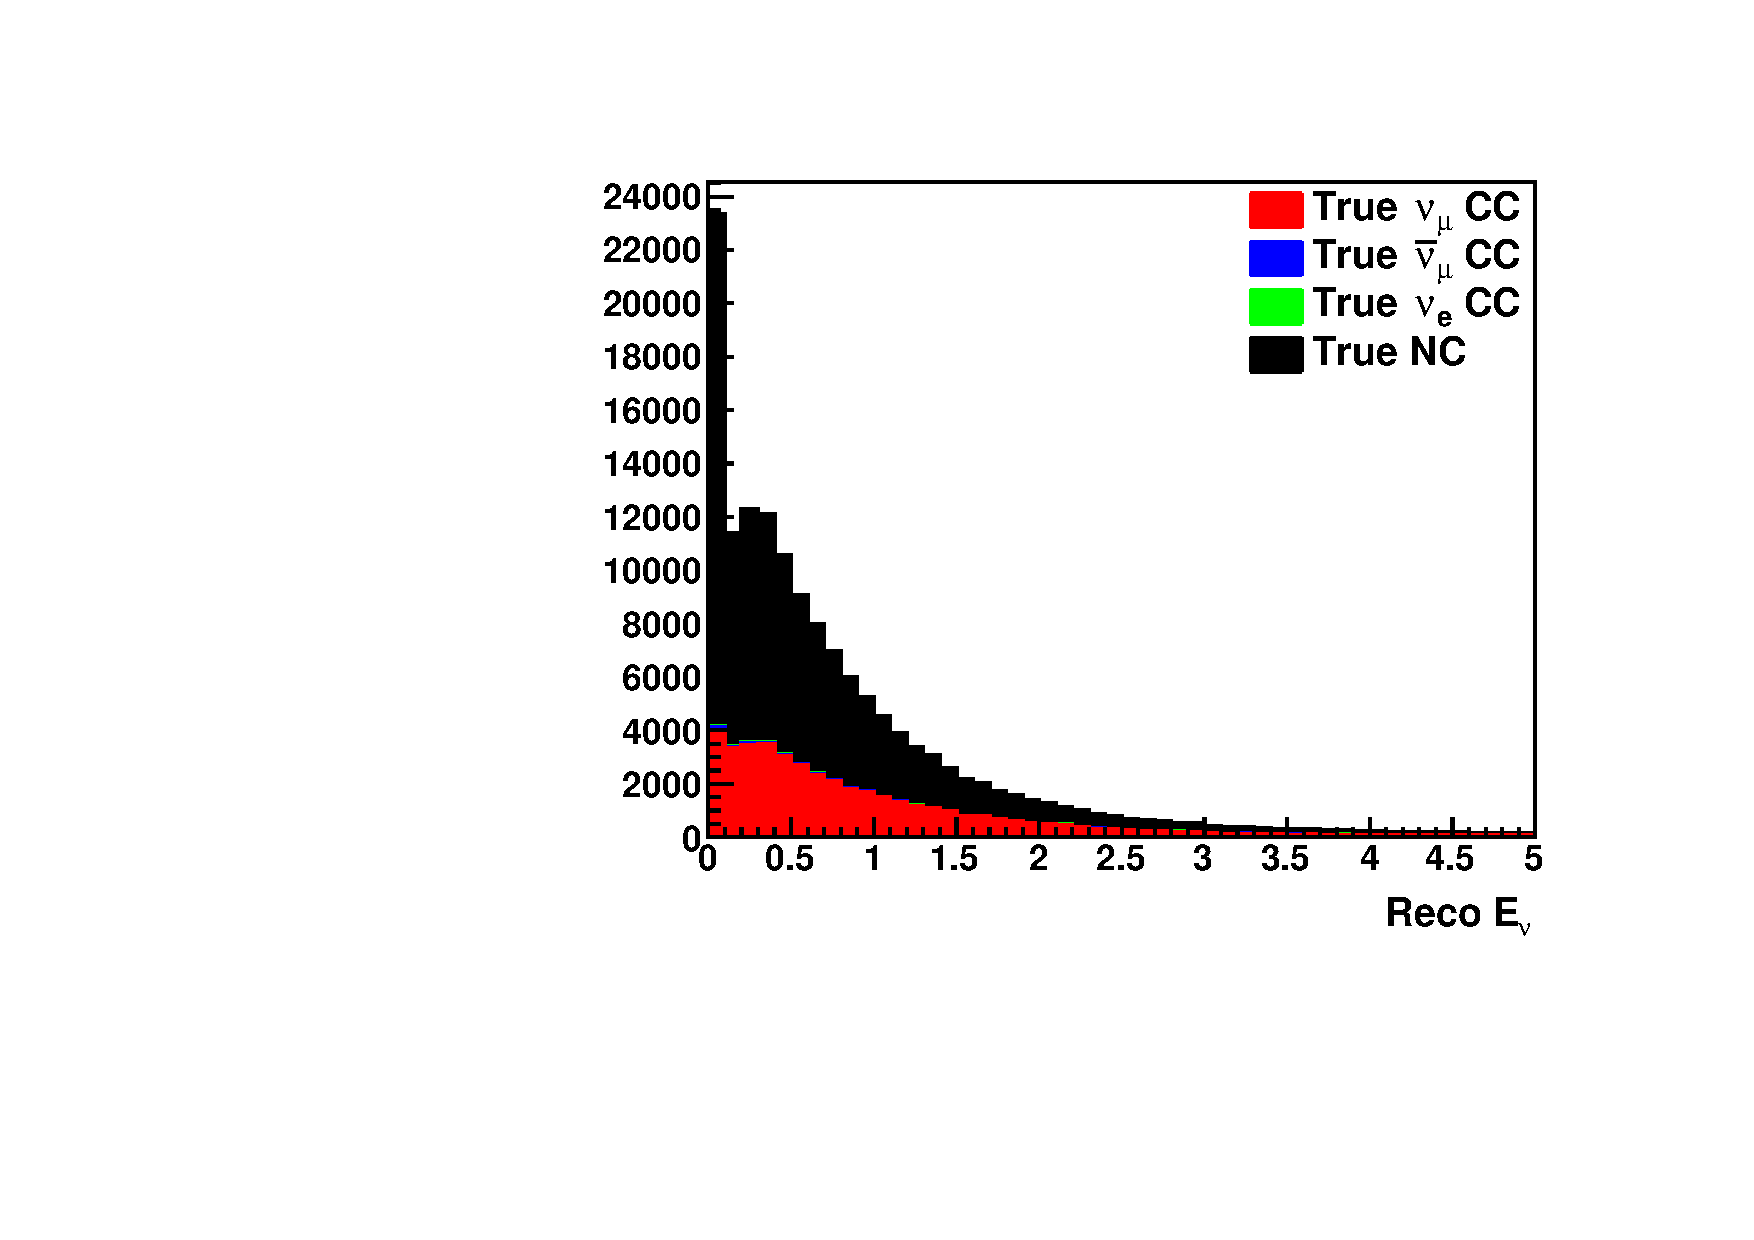
\includegraphics[width=0.3\textwidth]{recoE_NC.pdf}
\end{dunefigure}

In addition to the CC event selections, neutrino-electron elastic scattering is also selected. Measurements of neutrino-nucleus scattering are sensitive to the product of the flux and cross section, both of which are uncertain. This can lead to a degeneracy between flux and cross section nuisance parameters in the oscillation fit, and result in significant anti-correlations, even when the uncertainty on the diagonal component is small. One way to break this degeneracy is by including a sample for which the a priori cross section uncertainties are very small. 

Neutrino-electron scattering is a pure-electroweak process with calculable cross section at tree level. It is therefore possible to directly constrain the flux by measuring the event rate of $\nu+ e \rightarrow \nu +e$ and dividing by the known cross section. The final state consists of a single electron, subject to the kinematic limit 

\begin{equation}
1 - \cos \theta = \frac{m_{e}(1-y)}{E_{e}},
\end{equation}

where $\theta$ is the angle between the electron and incoming neutrino, $E_{e}$ and $m_{e}$ are the electron mass and total energy, respectively, and $y = T_{e}/E_{\nu}$ is the fraction of the neutrino energy transferred to the electron. For DUNE energies, $E_{e} \gg m_{e}$, and the angle $\theta$ is very small, such that $E_{e}\theta^{2} < 2m_{e}$.

The overall flux normalization can be determined by counting $\nu e \rightarrow \nu e$ events. Events can be identified by searching for a single electromagnetic shower with no other visible particles. Backgrounds from $\nu_{e}$ charged-current scattering can be rejected by looking for large energy deposits near the interaction vertex, which are evidence of nuclear breakup. Photon-induced showers from neutral-current $\pi^{0}$ events can be distinguished from electrons by the energy profile at the start of the track. The dominant background is expected to be $\nu_{e}$ charged-current scattering at very low $Q^{2}$, where final-state hadrons are below threshold, and $E_{e}\theta^{2}$ happens to be small. The background rate can be constrained with a control sample at higher $E_{e}\theta^{2}$, but the shape extrapolation to $E_{e}\theta^{2} \rightarrow 0$ is uncertain at the 10-20\% level.

For the DUNE flux, approximately 100 events per year per ton of fiducial mass ar expected with electron energy above 0.5 GeV. For a LAr TPC mass of 25 tons, this corresponds to 2500 events per year, or 12500 events in the full 5-year FHC run, assuming the ND stays on axis. Given the very forward signal, it may be possible to expand the fiducial volume to enhance the rate. The statistical uncertainty on the flux normalization from this technique is expected to be $\sim$1\%.

To evaluate the impact of neutrino-electron scattering, a dedicated high-statistics signal-only sample is generated. Due to the simple nature of the signal, it is possible to estimate backgrounds without a full detector simulation. A single electromagnetic shower (electron, positron or photon) is required. To reject $\pi^{0}$ events with clearly-identifiable second photons, no additional showers over 50 MeV are allowed.

Charged-current $\nu_{e}$ interactions can be rejected when there is evidence of nuclear breakup in the form final-state charged hadrons. A conservative cut of 40 MeV total charged hadron kinetic energy is applied. For a single proton, this corresponds to $\sim$ 1 cm of track length, which will leave energy on two or three readout pads and be easily identified. Finally, a cut requiring low $E_{e}\theta_{e}^{2}$ isolates the $\nu+e$ signal. Alternatively, templates in $(E_{e}, \theta_{e}$ can be formed, and the unique shape of the signal can be used in a fit to extract the flux normalization.

DUNE-PRISM details

\begin{table}
\begin{tabular}{ l l || c c | c || c c | c | c || c }
\multirow{3}{*}{Offset} & \multirow{3}{*}{$10^{19}$POT} & \multicolumn{7}{c||}{CCInc} & NCInc \\
\cline{3-10}
& & \multicolumn{3}{c||}{$\mu$ contained} & \multicolumn{3}{c|}{$\mu$ exit, $\textrm{T}_{\mu}^\textrm{\tiny exit} > 50 \textrm{MeV}$} & \multirow{2}{*}{$\nu_\textrm{e}$} & \multirow{2}{*}{$\nu_{\mu}$} \\
& & $\nu_{\mu}$ & $\epsilon_{\nu_{\mu},\textsc{cc}}$ & $\bar{\nu}_{\mu}$/$\nu_{\mu}$ & $\nu_{\mu}$ & $\epsilon_{\nu_{\mu},\textsc{cc}}$ & $\bar{\nu}_{\mu}$/$\nu_{\mu}$ & & \\ \hline
 0~m  &  55  & 6.6E5 & 3\% & 1\% & 5.3E6 & 22\% & 3\% & 6.2E4 & 1.8E6 \\
 3~m  &  4.58  & 5.5E4 & 3\% & 1\% & 4.1E5 & 22\% & 3\% & 5.0E3 & 1.4E5  \\
 6~m  &  4.58  & 5.8E4 & 4\% & 1\% & 3.0E5 & 22\% & 4\% & 4.3E3 & 1.1E5 \\
 9~m  &  4.58  & 6.0E4 & 7\% & 2\% & 1.9E5 & 22\% & 4\% & 3.4E3 & 7.5E4 \\
 12~m  &  4.58  & 5.9E4 & 12\% & 3\% & 1.1E5 & 22\% & 5\% & 2.5E3 & 5.2E4 \\
 15~m  &  4.58  & 5.4E4 & 18\% & 3\% & 6.2E4 & 20\% & 6\% & 2.2E3 & 3.7E4 \\
 18~m  &  4.58  & 4.6E4 & 22\% & 4\% & 3.8E4 & 18\% & 8\% & 1.7E3 & 2.7E4 \\
 21~m  &  4.58  & 3.9E4 & 27\% & 5\% & 2.5E4 & 17\% & 9\% & 1.4E3 & 2.1E4 \\
 24~m  &  4.58  & 3.1E4 & 30\% & 6\% & 1.7E4 & 16\% & 9\% & 1.2E3 & 1.6E4 \\
 27~m  &  4.58  & 2.6E4 & 32\% & 7\% & 1.2E4 & 15\% & 10\% & 9.8E2 & 1.3E4 \\
 30~m  &  4.58  & 2.1E4 & 33\% & 7\% & 9.6E3 & 16\% & 12\% & 8.3E2 & 1.0E4 \\
 33~m  &  4.58  & 1.7E4 & 35\% & 8\% & 7.5E3 & 15\% & 13\% & 7.6E2 & 8.3E3 \\
 36~m  &  4.58  & 1.2E4 & 35\% & 8\% & 6.1E3 & 16\% & 15\% & 6.7E2 & 6.6E3 \\
\hline
\hline
\multicolumn{2}{c||}{Totals} & $\nu_{\mu}$ & --- & $\bar{\nu}_{\mu}$ & $\nu_{\mu}$ & --- & $\bar{\nu}_{\mu}$ & $\nu_\textrm{e}$ & $\nu_{\mu}$ \\ \hline
 All  &  110  & 1.1E6 & --- & 1.6E4 & 6.5E6 & --- & 2.2E5 & 8.7E4 & 2.3E6 \\
\end{tabular}

\caption{The selected event rates for a year-long, neutrino-mode run plan. The wrong sign fraction, intrinsic electron neutrino and neutral current event rates are also shown. In all cases, the hadronic containment cut is applied, and the (anti-)muon neutrino events are separated into two samples depending on the containment topology of the final state muon.}
\label{table:evrates_LAR}
\end{table}
